%!TEX root = ../Thesis.tex

% 1.1 Background
% The background sets the general tone for your thesis. It should make a good impression and convince the reader why the theme is important and your approach relevant. Even so, it should be no longer than necessary.

% What is considered a relevant background depends on your field and its traditions. Background information might be historical in nature, or it might refer to previous research or practical considerations. You can also focus on a specific text, thinker or problem.

% Academic writing often means having a discussion with yourself (or some imagined opponent). To open your discussion, there are several options available. You may, for example:

% refers to a contemporary event
% outline a specific problem; a case study or an example
% review the relevant research/literature to demonstrate the need for this particular type of research
% If it is common in your discipline to reflect upon your experiences as a practitioner, this is the place to present them. In the remainder of your thesis, this kind of information should be avoided, particularly if it has not been collected systematically.

% Tip: Do not spend too much time on your background and opening remarks before you have gotten started with the main text.





\section{Background}
Coming from the field of telecommunication, through microwave engineering and electrical systems in satellites in last years I have focused on electric cars. After taking classes on electric vehicles I had my first practical experience by correcting the wire harness of converted to electric off-road car. Afterwards, I worked on electric conversion of car towards racing application.

Both systems, however, took an approach to use already designed solutions and did not require additional control units.

In by this thesis I got engaged into more ambitious project and took responsibility for main control unit.

In the following sections I will give brief insight into technical topics relevant to the final implementation.

\subsection{CAN}
Majority of communication from/to central control unit is realised based on Control Area Network (CAN) common communication protocol used mostly in automotive applications. It has been used within so far the most common version of psychical layer described in ISO11898-2 and popularly called high speed CAN.

In this standard both ends of the bus needs to be terminated to avoid signal reflections and the speed is reaching up to 1Mbit/s.

\paragraph{CAN Frame}
In this protocol each arbitrary data needs to be encapsulated into frames, each capable of transmitting variable number of bytes (up to 8 per frame).
Can frames consist of following fields:
\begin{table}[H]
\begin{tabular}{|p{0.2\textwidth}|p{0.13\textwidth}|p{0.58\textwidth}|}
\hline
\textbf{Filed} &\centering \textbf{Number of bits} &\textbf{Description} \\
\hline
Start-of-frame &\centering 1 & Denotes the start of frame transmission \\
\hline
Identifier &\centering 11 & A (unique) identifier which also represents the message priority \\
\hline
Remote transmission request &\centering 1 & Must be dominant for data frames and recessive for remote request frames \\
\hline
Identifier\newline extension bit &\centering 1 & Must be dominant for base frame format with 11-bit identifiers \\
\hline
Reserved bit &\centering 1 & Reserved bit. \\
\hline
Data length code &\centering 4 & Number of bytes of data (0–8 bytes) \\
\hline
Data field &\centering 0–64\newline (0-8 bytes) & Data to be transmitted\newline (length in bytes dictated by DLC field)\\
\hline
CRC &\centering 15 & Cyclic redundancy check\\
\hline
CRC delimiter &\centering 1 & Must be recessive\\
\hline
ACK slot &\centering 1 & Transmitter sends recessive and any receiver can assert a dominant\\
\hline
ACK delimiter &\centering 1 & Must be recessive\\
\hline
End-of-frame &\centering 7 & Must be recessive\\
\hline
\end{tabular}
\end{table}\todo{Source!}\footnote{Since CAN version 2.0 messages can be sent with 11 or 29 bit IDs. however, for simplicity I will just consider usage of 11 bit identifiers (they differ just by the number of bits in this field).}

It is multimaster asynchronous protocol and for proper operation requires each device to monitor the bus all the time (also during sending). So due to the fact that 0 is dominant, whenever two messages starts to sent in the same time the one which first sends 1 but is reading 0 stops sending immediately. Effectively, prioritising messages with lower IDs.

What is also worth to point out is that each CAN frame introduces protocol overhead of about 44bits per frame \footnote{Although, caring information message ID were included into message overhead calculation as in majority of cases it could be reduced to just a few bits, on the other hand we might expect additional bits due to bit stuffing(for each 4 bits with the same sign additional one is added)}.

\subsubsection{CANOpen}
It is an higher level of abstraction over the CAN (capable of working with variety of versions). The objective of this additional layer is to standardise format of the data as the original CAN protocol gives complete flexibility in the matter. 
In CANOpen message IDs consist of first 4 bits being a function ID and 7 bits representing device code (node ID). In this way the limitations was twisted around, in basic CAN network 2048 messages can be recognised, where CANOpen focuses on per device ID therefore changing limitation to 127 devices on the bus \footnote{on 7bits 128 devices could have own ID, however, ID equal to zero is used as broadcast channel}.

\begin{table}[]
    \centering
    \begin{tabular}{|p{0.28\textwidth}|p{0.3\textwidth}|p{0.3\textwidth}|}
        \hline
        \textbf{Communication object} & \textbf{COB-ID(s) hex} & \textbf{Slave nodes} \\
        \hline
        NMT node control & 000 & Receive only \\
        \hline
        Sync & 080 & Receive only \\
        \hline
        Emergency & 080 + NodeID & Transmit \\
        \hline
        TimeStamp & 100 & Receive only \\
        \hline
        PDO & 180 + NodeID & Transmit PDO1 \\
            & 200 + NodeID & Receive PDO1 \\
            & 280 + NodeID & Transmit PDO2 \\
            & 300 + NodeID & Receive PDO2 \\
            & 380 + NodeID & Transmit PDO3 \\
            & 400 + NodeID & Receive PDO3 \\
            & 480 + NodeID & Transmit PDO4 \\
            & 500 + NodeID & Receive PDO4 \\
        \hline
        SDO & 580 + NodeID & Transmit \\
            & 600 + NodeID & Receive \\
        \hline
        NMT node monitoring & 700 + NodeID & Transmit \\
        \hline
        LSS & 7E4 & Transmit \\
            & 7E5 & Receive \\
        \hline
    \end{tabular}
    \caption{Caption}
    \label{tab:my_label}
\end{table}\todo{Source!}

Addressing each device allows a variety of possibilities. It has been a base to establish protocol allowing to read/write data to device.
This functionality has been called "servicing data object" (SDO) and follows hierarchical addressing where at first device is chosen then certain parameter and possibly its sub-index. Although, it introduces an overhead, for basic parameters setting most likely there is no need for especially high throughput. 

In case that overhead is not tolerable CANOpen allows to map data in dictionary into "process dictionary object" (PDO). These are messages acting in the same way as raw CAN, being at the same time easily adjustable and having set of triggering methods.
Tigers included into this specification are: value change; timer overflow; device internal event; respond to request; respond to synchronisation message (SYNC).

\begin{wrapfigure}{L}{0.33\textwidth}
    \begin{center}
       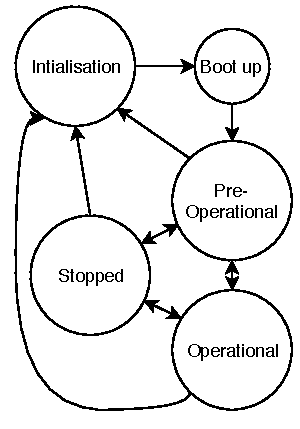
\includegraphics[width=0.3\textwidth]{figures/CANOpen_NMT}
    \end{center}
    \caption{Device states described in CANOpen specification}
    \label{fig:CANOpen NMT}
\end{wrapfigure}
Beside exchange of data CANOpen protocol describes a way to control basic device states. By messages referred as "Network Management" (NMT) one can read device state and send commands to change it. The states and all possible transitions are shown in figure \ref{fig:CANOpen NMT}.



% \section{Steering}
% \section{Torque vectoring / load sharing}
% \chapter{Existing solutions/ compare to IC vehicles}
% Literature review on recent developments within the topic and techniques used in combustion engine cars